% Date : April 1, 2020
% Author : 
% Subhankar Mishra
% School of Computer Sciences 
% NISER

\documentclass[12pt,a4paper]{report}
\setlength{\oddsidemargin}{0.25in}
\setlength{\evensidemargin}{0.15in}
\setlength{\topmargin}{0.3in}
\setlength{\textwidth}{6.0in}
\setlength{\textheight}{8.5in}
\usepackage{amsmath,amssymb}
\usepackage{graphics}
\usepackage{lscape,graphicx}
\usepackage{amsfonts}
\usepackage{longtable}
\usepackage{epsfig}
\usepackage{float}
\usepackage{rotating}

\usepackage{fancyhdr}
\usepackage{listings}
\usepackage{xcolor}

\definecolor{codegreen}{rgb}{0,0.6,0}
\definecolor{codegray}{rgb}{0.5,0.5,0.5}
\definecolor{codepurple}{rgb}{0.58,0,0.82}
\definecolor{backcolour}{rgb}{0.95,0.95,0.92}

\lstdefinestyle{mystyle}{
	backgroundcolor=\color{backcolour},   
	commentstyle=\color{codegreen},
	keywordstyle=\color{magenta},
	numberstyle=\tiny\color{codegray},
	stringstyle=\color{codepurple},
	basicstyle=\ttfamily\footnotesize,
	breakatwhitespace=false,         
	breaklines=true,                 
	captionpos=b,                    
	keepspaces=true,                 
	numbers=left,                    
	numbersep=5pt,                  
	showspaces=false,                
	showstringspaces=false,
	showtabs=false,                  
	tabsize=2
}

\lstset{style=mystyle}
\usepackage{hyperref}
\hypersetup{
	colorlinks=true,
	linkcolor=blue,
	filecolor=blue,
	citecolor = blue,      
	urlcolor=cyan,
}
\usepackage{siunitx}
\DeclareSIUnit \h {\mbox{$h$}}
\DeclareSIUnit \parsec {pc}
\usepackage[
backend=biber,
citestyle=authoryear,
bibstyle=science,
]{biblatex}
\AtEveryCitekey{\clearfield{title}}
\addbibresource{reference.bib}
\setlength{\headheight}{15pt}
\usepackage[titletoc]{appendix}
\usepackage[english]{babel}
\addto{\captionsenglish}{\renewcommand{\bibname}{References}}

\usepackage{titlesec}
\titlespacing*{\chapter}{0pt}{0pt}{0pt}
\titleformat{\chapter}[display]{\normalfont\huge\bfseries}{\chaptertitlename\ \thechapter}{20pt}{\Huge}

%%%%%%%%%%%%%%%%%%%%%%%%%%%%%%%%%%%%%%%%%%
%%%  macro for margin change
\newenvironment{changemargin}[2]{%
\begin{list}{}{%
%\setlength{\topsep}{0pt}%
\setlength{\leftmargin}{#1}%
\setlength{\rightmargin}{#2}%
%\setlength{\listparindent}{\parindent}%
%\setlength{\itemindent}{\parindent}%
%\setlength{\parsep}{\parskip}%
}%
\item[]}{\end{list}}
%%%%%%%%%%%%%%%%%%%%%%%%%%%%%%%%%%%%%%%%%%

\begin{document}
\begin{titlepage}

\begin{center}

\textup{\small {\bf Summer Internship Project} \\ Report}\\[0.3in]

% Title
\Large \textbf {The Chemical Picture of Protoplanetary Disk Evolution}\\[0.7in]


       

% Submitted by
\normalsize Submitted by \\[0.2in]
\textbf{Maitrey Sharma}\\
Fourth Year Integrated M.Sc.\\
National Institute of Science Education and Research, Bhubaneshwar\\

\vspace{.2in}
Under the guidance of\\[0.2in]
\textbf{Dr. Liton Majumdar}\\
Reader-F

School of Earth and Planetary Sciences 

National Institute of Science Education and Research, Bhubaneshwar



\vspace{.3in}

% Bottom of the page

\includegraphics[width=0.3\textwidth]{logo1.jpg}\\[0.1in]
\Large{School of Earth and Planetary Sciences}\\
\normalsize
\textsc{National Institute of Science Education and Research}\\
Bhubaneshwar \\
\vspace{0.2cm}
Summer Internship 2023

\end{center}

\end{titlepage}

\pagenumbering{roman}
\baselineskip=20pt
%
\begin{center}
{\large {\bf DEDICATION (OPTIONAL)}} 
\end{center}


\begin{center}
{\bf DECLARATION}
\end{center}

I hereby declare that I am the sole author of this report in  fulfillment of the requirements for Summer Internship from National Institute of Science Education and Research (NISER). I authorize NISER to lend this report to other institutions or individuals for the purpose of scholarly research.

\vskip1.0in

\hspace*{3.5in} {Signature of the Student} \\
\hspace*{3.5in} {Date:}

\vskip1.0in
\vskip1.0in

The work reported in the report entitled .......................................................  was carried out under my supervision, in the school of ............................................... at NISER, Bhubaneswar, India.

\vskip1.0in

\hspace*{3in} {Signature of the project supervisor} \\
\hspace*{3in} {School:}\\
\hspace*{3in} {Date:}
%\include{stat}
%\include{cert1}
%\begin{center}
{\bf ACKNOWLEDGEMENTS}
\end{center}

I wish to thank xxx......


\vspace{2in}
\begin{abstract}


\end{abstract} 

\clearpage
\fancyfoot{}      % Delete current footer settings

\pagestyle{fancyplain}
 \renewcommand{\chaptermark}[1]{\markboth{\thechapter\ #1}{\thechapter\ #1}} % remember chapter title
 \lhead[\fancyplain{}{}]{\fancyplain{}{}}
 \rhead[\fancyplain{}{}]{\fancyplain{}{\em\leftmark }}
 \renewcommand{\headrulewidth}{0.3pt}
 \cfoot{\rm\thepage} % page number

\baselineskip=12pt
\tableofcontents
\clearpage
%\listoffigures
\clearpage
%\listoftables 
\clearpage
\pagenumbering{arabic}
\baselineskip=15pt
\chapter{\label{intro}Introduction}

\setcounter{equation}{0}
\setcounter{table}{0}
\setcounter{figure}{0}

\vspace{5mm}
The Universe came to be from an homogeneous hot dense phase, a gravitational singularity where spacetime breaks down catastrophically to an heterogeneous vast and sparse state. Different types of cosmological formations took place as it cooled down and expanded over the course of billion years after the Big Bang. \textit{Structure formation}, as it is called, is the formation of galaxies, galactic clusters and larger structures from small early density fluctuations. The study of these structures provide immense insight into the early Universe. 
Galactic formation and evolution is, thus, one of the most important areas of study of cosmology. Galaxies are diverse, with each class having their own set of properties and what they can reveal about the early Universe.
\par
In this work we will first build our premise towards a special type of galaxies, defined by where they are found, discuss why they are so crucial and what probes we can use to study them. After that we will discourse the objective of this work, the methodologies used and then finally discuss the results and draw conclusions. 
\section{Cosmic Voids}
Cosmic voids are vast spaces between galaxy filaments (the largest structures in the Universe) which contain very few or no galaxies. Voids are enormous regions with sizes in the range of 20-50 \si{\per \h \mega \parsec} that are practically devoid of any galaxy, usually roundish in shape and occupying the major share of space in the Universe. There are a variety of reasons the study of voids is relevant to our understanding of the Universe (\cite{van_de_weygaert_cosmic_2011}).
\begin{enumerate}
	\item They are a prominent aspect of the Megaparsec Universe, instrumental in the spatial organization of the Cosmic Web.
	\item Voids contain a considerable amount of information on the underlying cosmological scenario and on global cosmological parameters. Notable cosmological imprints are found in the outflow velocities and accompanying redshift distortions (\cite{dekel_omega_1994}, \cite{martel_simulation_1989}, \cite{ryden_voids_1996}). Also their intrinsic structure, shape and mutual alignment are sensitive to the cosmology, including that of dark energy (\cite{park_void_2007}; \cite{lee_constraining_2009}; \cite{platen_alignment_2008}).
	\item The pristine low-density environment of voids represents an ideal and pure setting for the study of galaxy formation and the influence of cosmic environment on the formation of galaxies.
\end{enumerate}
The last is particularly interesting and forms the basis of this work as we will see in the next section.
\section{Void Galaxies}
A void galaxy is a galaxy located in a cosmological void. Few galaxies exist in voids; most are located in sheets, walls and filaments that surround voids and supervoids. These galaxies are predominately low-mass and often brimming with star formation (\cite{singari_detection_2018}). These galaxies are subject to dynamics that are unique to these underdense regions. They are generally late type disk galaxies that are gas rich, star-forming systems lying mainly on the blue cloud of galaxy evolution (\cite{beygu_void_2017}; \cite{kreckel_only_2011})
\par
Several surveys, thus, have been conducted in past few years to systematize the study of these galaxies, such as the Void Galaxy Survey (VGS) and Galaxy and Mass Assembly (GAMA) survey. So far we have established that void galaxies present a unique and interesting case to study galaxy formation, what effects the neighboring environment can have on it and the cosmos as a whole. For this work, we will be using a public catalog\footnote{\url{http://www.physics.drexel.edu/~pan/VoidCatalog/}} prepared by \citeauthor{pan_cosmic_2012} (\cite*{pan_cosmic_2012}).
\section{Cosmic Microwave Background}
Cosmic microwave background, the relic radiation from the Universe is mostly isotropic, but not quite. Therefore, precise measurements of anisotropies in temperature, polarization and spectrum of the CMB are of immense interest in cosmology and it is the reason massive projects such as the Planck Collaboration exist.
\par 
CMB spectral distortions are tiny departures of the average cosmic microwave background (CMB) frequency spectrum from the predictions given by a perfect black body, and they were first starting with the seminal papers of Yakov B. Zeldovich and Rashid Sunyaev (\cite{sunyaev_small-scale_1970}).
\section{The Sunyaev-Zeldovich Effect and the Circumgalactic Medium}
The Sunyaev–Zeldovich effect (abbreviated as the SZ effect from here) is the spectral distortion of the cosmic microwave background (CMB) through inverse Compton scattering by high-energy electrons in galaxy clusters, in which the low-energy CMB photons receive an average energy boost during collision with the high-energy cluster electrons.
\par 
If this distortion results from a large number of high energy electrons is known as the thermal Sunyaev–Zeldovich (tSZ) effect. The tSZ effect is the best probe of the large scale distribution of the diffuse hot gas component of our Universe, with temperature $T > 10^6 \si{\kelvin}$. The tSZ effect has been recently used for detecting the circum-galactic medium (CGM) around massive galaxies usually for locally bright galaxies of stellar masses larger than $ 10^{11} \textup{M}_{\odot} $ (\cite{planck_collaboration_planck_2013}).
\par 
Since these void galaxies are isolated and have low stellar masses, they are ideal for studying the hot gas due to stellar feedback lying within the CGM of galaxies. In this work we will discuss the process of constraining our data of void galaxies from the catalog (\cite{pan_cosmic_2012}) and then using stacking techniques with the all-sky Planck $ y $-map.
%\baselineskip 24pt


    




\chapter{\label{method}Methods}

\setcounter{equation}{0}
\setcounter{table}{0}
\setcounter{figure}{0}
%\baselineskip 24pt


    




\chapter{\label{results}Results and Discussion}
After implementing the code, the filter can be generated as per user's requirements. Some plots are included with did not use the filter but represent the results which are obtained by stacking the void galaxies. MILCA refers to Modified Internal Linear Component Algorithm (\cite{hurier_milca_2013}), which is a internal linear combination (ILC) method used to extract the CMB emission from the WMAP multifrequency data courtesy projects like the Planck survey. NILC stands for Needlet Internal Linear Combination (\cite{remazeilles_cmb_2011}), a different technique used for same purpose.
\begin{figure}[h!]
	\centering
	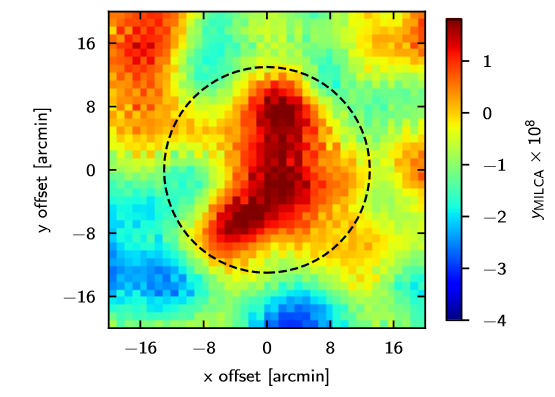
\includegraphics{fig2.png}
	\caption{The normalized stacked $ y $ MILCA map at void galaxy locations at all z in our sample over $ 51\% $ sky mask.}
\end{figure}
\begin{figure}[h!]
	\centering
	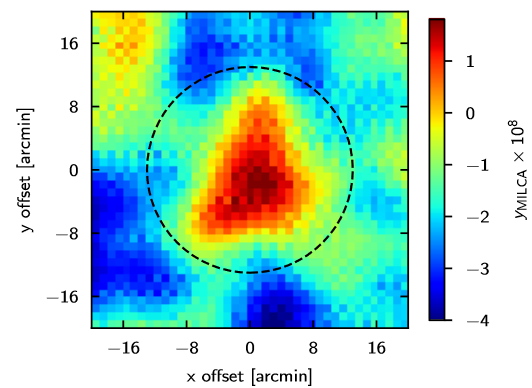
\includegraphics{fig3-1.png}
	\caption{The normalized stacked $ y $ MILCA map at void galaxy locations at $ z > 0.04 $ in our sample over $ 51\% $ sky mask.}
\end{figure}
\begin{figure}[h!]
	\centering
	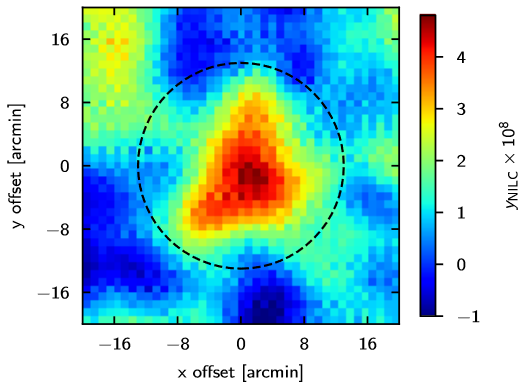
\includegraphics{fig3-2.png}
	\caption{The normalized stacked $ y $ NILC map at void galaxy locations at $ z > 0.04 $ in our sample over $ 51\% $ sky mask.}
\end{figure}
Using the filter, similar stacking plots can be obtained. The filtering will aid in removing unwanted galaxies, that are too near the void walls. 
\setcounter{equation}{0}
\setcounter{table}{0}
\setcounter{figure}{0}
%\baselineskip 24pt


    




%\chapter{\label{summary}Summary and Conclusions}

\setcounter{equation}{0}
\setcounter{table}{0}
\setcounter{figure}{0}
%\baselineskip 24pt


    




%%\clearpage
%\addcontentsline{toc}{chapter}{Appendices}
\begin{appendices}
\chapter{\label{appendix}(Optional)}
\end{appendices}


\setcounter{equation}{0}
\setcounter{table}{0}
\setcounter{figure}{0}
%\baselineskip 24pt


    




%\newline
Birkinshaw M. 1999. Physics Reports. 310(2–3):97–195
\newline
Emritte MS, Colafrancesco S, Marchegiani P. 2016. J. Cosmol. Astropart. Phys. 2016(07):031–031
\newline
Fielding D, Quataert E, McCourt M, Thompson TA. 2017. Mon. Not. R. Astron. Soc. 466(4):3810–26
\newline
Haider M, Steinhauser D, Vogelsberger M, Genel S, Springel V, et al. 2016. Mon. Not. R. Astron. Soc. 457(3):3024–35
\newline
Hogg DW. 2000
\newline
Hurier G, Macías-Pérez JF, Hildebrandt S. 2013. A&A. 558:A118
\newline
Kreckel K, Platen E, Aragón-Calvo MA, van Gorkom JH, van de Weygaert R, et al. 2012. The Astronomical Journal. 144(1):16
\newline
Luzzi G, Shimon M, Lamagna L, Rephaeli Y, De Petris M, et al. 2009. ApJ. 705(2):1122–28
\newline
Pan DC, Vogeley MS, Hoyle F, Choi Y-Y, Park C. 2012. Monthly Notices of the Royal Astronomical Society. 421(2):926–34
\newline
Remazeilles M, Delabrouille J, Cardoso J-F. 2011. Monthly Notices of the Royal Astronomical Society. 410(4):2481–87
\newline
Singari B, Ghosh T, Das M, Ma Y-Z, Tanimura H. , p. 6
\newline
Sunyaev RA, Zeldovich YaB. 1970. Astrophys Space Sci. 7(1):3–19
\newline
Tanimura H, Aghanim N, Douspis M, Beelen A, Bonjean V. 2019. A&A. 625:A67
\newline
Tumlinson J, Peeples MS, Werk JK. 2017. Annu. Rev. Astron. Astrophys. 55(1):389–432
\newline
van de Weygaert R, Kreckel K, Platen E, Beygu B, van Gorkom JH, et al. 2011. , pp. 17–24
\newline
van de Weygaert R, Platen E. 2011. Int. J. Mod. Phys. Conf. Ser. 01:41–66
%}
\nocite{*}

\bibliography{reference.bib}
\addcontentsline{toc}{chapter}{Bibliography}
\end{document}
